% Two overlapping open sets U and V, whose sections glue on the overlap.
% Source: book/tex/alg-geom/sheaves.tex (§ the gluing axiom).
\documentclass[border=2mm]{standalone}
\usepackage{tikz}
\usepackage{amssymb}
\begin{document}
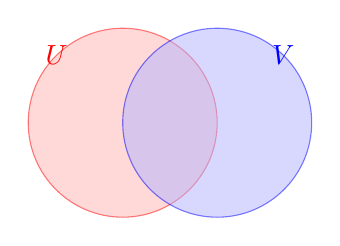
\begin{tikzpicture}[scale=1.2]
  \filldraw[red!30, opacity=0.5, draw=red] (-0.5,0) circle (1);
  \filldraw[blue!30, opacity=0.5, draw=blue] (0.5,0) circle (1);
  \node[red] at (-1.2,0.72) {$U$};
  \node[blue] at (1.2,0.72) {$V$};
\end{tikzpicture}
\end{document}
